\documentclass[11pt,oneside,a4paper]{article}

\usepackage{authblk}
\usepackage{hyperref}
\usepackage{graphicx}
\usepackage{bm}
\usepackage{mathtools,esint}
\usepackage{amssymb}
\usepackage{xcolor}
\usepackage{listings}

\usepackage[margin=2.0cm]{geometry} % margins %

\definecolor{cident}{rgb}{0.0,0.0,0.0}
\definecolor{ckeyw}{rgb}{0,0,0.8}
\definecolor{ccomm}{rgb}{0,0.8,0}
\definecolor{cstr}{rgb}{0.8,0,0}
\definecolor{myyellow}{rgb}{0.99,0.76, 0.0}
\definecolor{mymagenta}{rgb}{1.0, 0.0, 1.0}

\lstset{language=[LaTeX]{TeX},
  basicstyle=\normalsize\ttfamily,
  keywordstyle=\color{ckeyw}\bfseries,
  identifierstyle=\color{cident}\bfseries,
  commentstyle=\color{ccomm},
  stringstyle=\color{cstr},
  showstringspaces=false,
  breaklines=true,
  breakatwhitespace=true,
  tabsize=2,
  mathescape = false,
  columns=flexible,
  escapeinside={<@}{@>}
%   numbers=left,
%   stepnumber=1,
%   firstnumber=1,
%   numberfirstline=true,
  }
\setlength\parindent{0pt}

\begin{document}

\title{PH388 Project \#: XYZ}

\author[1]{Oliver Henrich}
\author[2]{Oliver Henrich}
\affil[1]{Group Zombies, \href{mailto:oliver.henrich@strath.ac.uk}{oliver.henrich@strath.ac.uk}}
\affil[2]{Group Zombies, \href{mailto:oliver.henrich@strath.ac.uk}{oliver.henrich@strath.ac.uk}}

\date{\today}

\maketitle

\section{Introduction}

One of the greatest, but rather unknown physicists was James Clerk Maxwell (see Fig. \ref{jcm}), who unified several concepts of the electromagnetic field and predicted the existence of electromagnetic waves \cite{maxwell}.

\begin{figure}[htpb!]
\begin{center}
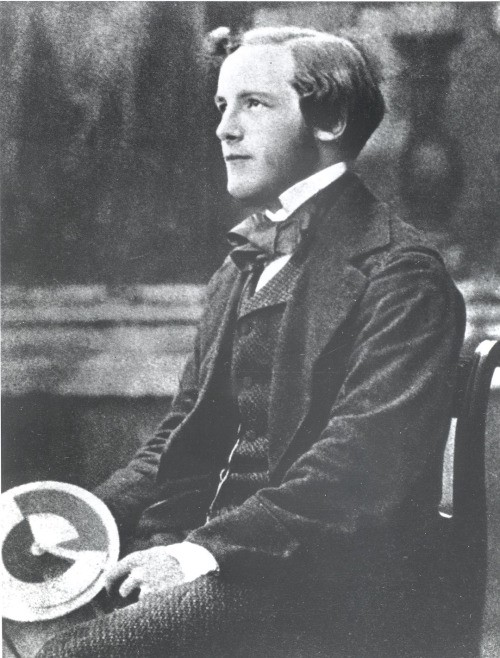
\includegraphics[height=0.25\textwidth]{jcm-young.jpg}
\hspace{0.5cm}
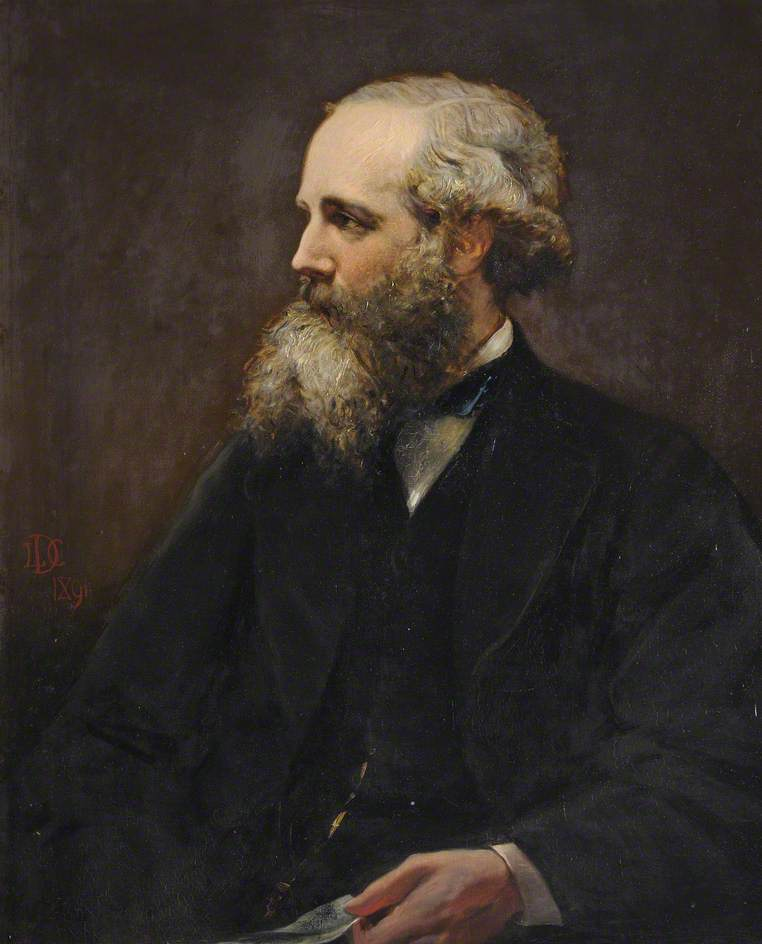
\includegraphics[height=0.25\textwidth]{jcm-painting.jpg}
\caption{James Clerk Maxwell as a young man at Trinity College, Cambridge, holding one of his colour wheels (left); Maxwell as Fellow of Trinity College (right)}\label{jcm}
\end{center}
\end{figure}

\section{Results}

In differential form the four Maxwell equations are
\begin{eqnarray}
\mbox{Gauss's law:}\hspace{0.5cm} \bm{\nabla}\cdot\mathbf{E}&=&\frac{\rho}{\epsilon_0}\nonumber\\
\mbox{Gauss's law for magnetism:}\hspace{0.5cm}  \bm{\nabla}\cdot\mathbf{B}&=&0\nonumber\\
\mbox{Maxwell-Faraday equation:}\hspace{0.5cm}  \bm{\nabla}\times\mathbf{E}&=&-\frac{\partial\mathbf{B}}{\partial t}\nonumber\\
\mbox{Amp\`ere's circuit law:}\hspace{0.5cm}  \bm{\nabla}\times\mathbf{B}&=&\mu_0\left(\mathbf{J}+\epsilon_0\frac{\partial\mathbf{E}}{\partial t}\right).\label{maxequ-diff}
\end{eqnarray}

In integral form they read
\begin{eqnarray}
\mbox{Gauss's law:}\hspace{0.5cm}  \oiint_{\partial V} \mathbf{E}\cdot d\mathbf{S}&=&\frac{1}{\epsilon_0}\iiint_V\rho dV\nonumber\\
\mbox{Gauss's law for magnetism:}\hspace{0.5cm}  \oiint_{\partial V} \mathbf{B}\cdot d\mathbf{S}&=&0\nonumber\\ 
\mbox{Maxwell-Faraday equation:}\hspace{0.5cm}  \oint_{\partial S} \mathbf{E}\cdot d\mathbf{l} &=&-\frac{d}{dt} \iint_S \mathbf{B}\cdot d\mathbf{S}\nonumber\\
\mbox{Amp\`ere's circuit law:}\hspace{0.5cm}  \oint_{\partial S} \mathbf{B}\cdot d\mathbf{l}&=&\mu_0\left(\iint_S \mathbf{J}\cdot d\mathbf{S} +\epsilon_0\frac{d}{dt}\iint_S \mathbf{E}\cdot d\mathbf{S}\right).\label{maxequ-int}
\end{eqnarray}

The quantities that appear therein are

\begin{table}[htbp!]
\begin{center}
\begin{tabular}{|c|c|c|}
\hline
Quantity & Name & SI Unit\\
\hline
$\mathbf{E}$ & electric field & $V \cdot m^{-1}$\\
\hline
$\mathbf{B}$ & magnetic flux density & $kg \cdot  A^{-1} \cdot s^{-2}$\\
\hline
$\rho$ & charge density & $A \cdot s$\\
\hline
$\mathbf{J}$ & current density & $A \cdot m^{-2}$\\
\hline
$\epsilon_0$ & vacuum permittivity & $8.85 \times 10^{-12} A^2 \cdot s^4 \cdot kg^{-1} \cdot m^{-3}$\\
\hline
$\mu_0$ & vacuum permeability & $1.25 \times 10^{-6} kg \cdot m \cdot s^{-2} \cdot A^{-2}$\\
\hline
\end{tabular}
\caption{Key to the notation of the Maxwell equations in vacuum: {\bf Bold} quantities represent vectors, whereas regular quantites are scalars. The unit of each quantity and the universal constants is given in the \textit{Syst\`eme International d'Unit\'e} (SI units)}
\end{center}
\end{table}

\section{Conclusions}

Neither the differential form Eqs.\ref{maxequ-diff} nor the integral form Eqs. \ref{maxequ-int} was given by Maxwell himself. The form commonly used today was a compact synthesis of Maxwell's 20 (scalar) equations in vector form by Oliver Heaviside \cite{heaviside}, one of the inventors of vector calculus. At Maxwell's time this mathematical concept has not yet been invented, making his discovery an even greater achievement (see Fig. \ref{me-modern-world}). 

\begin{figure}[htbp!]
\begin{center}
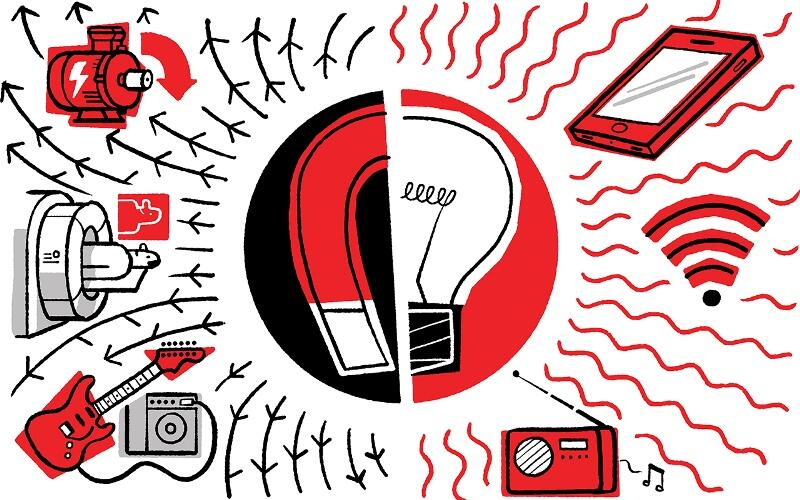
\includegraphics[width=0.45\textwidth]{maxwells-equations.jpg}
\caption{It is impossible to imagine our world today without Maxwell's equations.}\label{me-modern-world}
\end{center}
\end{figure}

\begin{thebibliography}{9}
\bibitem{maxwell} James Clerk Maxwell, A dynamical theory of the electromagnetic field, \textit{Phil. Trans. R. Soc.} \textbf{155}, 459–512 (1865).
\bibitem{heaviside} Oliver Heaviside, \textit{Electromagnetic Theory}, Vol. 3, "The Electrician" Printing and Publishing Company Ltd., London (1893).

\end{thebibliography}

\appendix

\section{Code Listings}

\subsection{JCMSaysHello.py}

\begin{lstlisting}[language=python]
from datetime import date

print('JCM says: \'Hello 21st Century World!\'')
today = date.today()
print('\'Today is %s, a good day to enjoy my equations!\'' % today)
\end{lstlisting}

\end{document}
